\documentclass[journal]{IEEEtran}

% ── Packages ──────────────────────────────────────────────────────────────────
\usepackage{cite}
\usepackage{amsmath,amssymb,amsfonts}
\usepackage{graphicx}
\usepackage{textcomp}
\usepackage{xcolor}
\usepackage{booktabs}
\usepackage{multirow}
\usepackage{url}
\usepackage{array}
\usepackage[hidelinks]{hyperref}
\usepackage{tabularx}
\usepackage{threeparttable}
\usepackage{tikz}
\usetikzlibrary{arrows.meta,positioning,shapes.geometric}

% ── Title & Authors ────────────────────────────────────────────────────────────
\begin{document}

\title{Low-Code AI Workflow Tools for ML Data Pipeline Automation:\\
A Comparative Study of n8n, Flowise, and Apache Airflow}

\author{Muhammad~Shoaib~Inksar and Sundas~Shahzeen%
  \thanks{Manuscript received Month XX, 2026; revised Month XX, 2026;
    accepted Month XX, 2026. Date of publication Month XX, 2026.
    This work was supported by the Department of Data Science,
    University of Management and Technology, Lahore, Pakistan.
    \emph{(Corresponding author: Muhammad Shoaib Inksar.)}}%
  \thanks{M.~S.~Inksar is with the Department of Data Science,
    University of Management and Technology, Lahore 54770, Pakistan
    (e-mail: m.shoaib@student.umt.edu.pk).}%
  \thanks{S.~Shahzeen is with the Department of Data Science,
    University of Management and Technology, Lahore 54770, Pakistan
    (e-mail: sundas.shahzeen@umt.edu.pk).}}

\markboth{IEEE ACCESS, VOL.~XX, NO.~XX, 2026}%
{Inksar \MakeLowercase{\textit{et al.}}: Low-Code AI Workflow Tools
  for ML Data Pipeline Automation}

\maketitle

% ── Abstract ──────────────────────────────────────────────────────────────────
\begin{abstract}
The increasing complexity of machine learning~(ML) systems in production
environments has amplified demand for reliable, automated data pipeline
solutions. Despite growing investment in ML infrastructure, a substantial
proportion of ML projects fail to reach deployment, largely due to
inadequate data engineering practices and the inherent complexity of
traditional workflow orchestration tools. The emergence of low-code
AI-native platforms---specifically n8n and Flowise---offers a compelling
alternative to code-centric orchestrators such as Apache Airflow. However,
no systematic empirical study has evaluated these platforms against one
another in the context of ML data pipeline automation. This paper presents
a comprehensive comparative study of n8n, Flowise, and Apache Airflow,
applied to automated ML data preprocessing pipelines. We implement five
identical preprocessing tasks---missing value imputation, duplicate
detection, data type conversion, outlier handling, and feature
normalization---across all three platforms using two benchmark datasets:
the UCI Adult Income dataset (48,842 instances, 15 features) and a
real-world smartphone specifications dataset (1,023 instances,
12 features). The evaluation employs six quantitative metrics---pipeline
setup time, development time, execution time, memory consumption, CPU
utilization, and operator count---alongside six qualitative dimensions
covering ease of installation, interface usability, error handling,
integration ecosystem, documentation quality, and scalability potential.
Results demonstrate that Flowise achieves the lowest execution time on
both datasets (0.160\,s and 0.017\,s on DS-A and DS-B, respectively),
outperforming Airflow by a factor of~5.1 on the large-scale dataset,
while n8n incurs the highest latency on large data (2.461\,s) due to
JavaScript engine overhead. All three tools achieve equivalent data
quality outcomes (100\% task completion), confirming that tool choice
affects development effort and runtime performance rather than
preprocessing correctness. Based on these findings, practical
tool-selection guidelines are derived for data engineers and ML
practitioners across varying expertise levels and deployment contexts.
All pipeline implementations are made publicly available to facilitate
reproducibility.
\end{abstract}

\begin{IEEEkeywords}
machine learning operations, workflow orchestration, data pipeline
automation, low-code AI, n8n, Flowise, Apache Airflow, MLOps,
comparative study, data engineering
\end{IEEEkeywords}


% ─────────────────────────────────────────────────────────────────────────────
\section{Introduction}
\label{sec:introduction}
% ─────────────────────────────────────────────────────────────────────────────

\IEEEPARstart{T}{he} rapid proliferation of machine learning~(ML)
applications across sectors such as healthcare, finance, manufacturing,
and e-commerce has fundamentally reshaped the demands placed on data
infrastructure. Organizations increasingly rely on ML-driven decision
systems that must ingest, clean, and transform large volumes of
heterogeneous data before model training or inference can occur. The
\textit{data pipeline}---the sequence of extraction, transformation, and
loading~(ETL) operations that prepares raw data for ML consumption---has
therefore emerged as a critical determinant of ML system reliability and
performance~\cite{sculley2015hidden}.

The consequences of inadequate pipeline management are well documented.
Sculley et al.~\cite{sculley2015hidden} established that data verification,
feature engineering, and pipeline glue code collectively constitute the
dominant source of \textit{technical debt} in production ML systems,
substantially outweighing the complexity of the model code itself.
Paleyes et al.~\cite{paleyes2023challenges} further demonstrated through
an analysis of industry case studies that data management failures---
including schema drift, missing value propagation, and undocumented
preprocessing inconsistencies---are among the leading causes of ML
deployment failures. Industry surveys reinforce this picture: as many as
85\% of ML models fail to transition from experimentation to production,
with data quality and pipeline reliability cited as primary
contributors~\cite{kreuzberger2023mlops}.

These challenges gave rise to the discipline of \textit{Machine Learning
Operations}~(MLOps), which systematizes the deployment, monitoring, and
maintenance of ML systems at scale~\cite{kreuzberger2023mlops,
symeonidis2022mlops, amershi2019software}. Within the MLOps stack,
\textit{workflow orchestration tools} play a foundational role: they
schedule and coordinate the individual preprocessing tasks that constitute
an end-to-end data pipeline, manage dependencies between those tasks,
handle failures gracefully, and expose observability interfaces for
monitoring pipeline health.

Apache Airflow~\cite{airflow2015}, introduced by Airbnb in 2014 and
subsequently adopted as an Apache Software Foundation top-level project,
has become the industry-standard tool for pipeline orchestration. Its
Directed Acyclic Graph~(DAG) abstraction enables complex, dependency-aware
scheduling through Python code. Despite its power, Airflow imposes a
significant operational burden: practitioners must author Python DAG files,
manage a multi-component deployment (webserver, scheduler, metadata database,
worker pool), and contend with a steep learning curve that can hinder
adoption among data scientists without strong software engineering
backgrounds~\cite{symeonidis2022mlops, shankar2022operationalizing}.

In response to these usability limitations, a new generation of
\textit{low-code} and \textit{AI-native} workflow platforms has emerged.
n8n is an open-source visual automation platform that enables pipeline
construction through a node-graph interface, requiring minimal programming
skill. Flowise, purpose-built for large language model~(LLM) orchestration,
introduces an agent-based paradigm in which AI components---including
language models, retrieval mechanisms, and custom tools---can be
embedded directly into data processing workflows. Both tools offer
graphical pipeline editors that contrast sharply with Airflow's code-first
approach. Together, they represent a fundamentally different philosophy:
prioritizing accessibility and rapid prototyping over the operational
sophistication expected in large-scale enterprise deployments.

Despite growing adoption of n8n and Flowise in industry settings, no
systematic empirical study has evaluated either platform against Apache
Airflow in the context of ML data pipeline automation. Existing comparative
studies of orchestration tools focus exclusively on code-first platforms
such as Prefect, Luigi, and Dagster, and do not account for the low-code
paradigm's distinct implications for development velocity, resource
efficiency, or data quality outcomes~\cite{symeonidis2022mlops,
goyal2023automated}. This gap is consequential: without principled,
evidence-based guidance, practitioners selecting workflow orchestration
tools must rely on marketing claims or anecdotal experience, risking
costly mismatches between tool capability and operational requirements.

This paper addresses this gap through a rigorous comparative evaluation.
We design and implement five identical ML data preprocessing tasks across
n8n, Flowise, and Apache Airflow, using two datasets of differing scale
and domain characteristics. The evaluation spans both quantitative
performance benchmarks and structured qualitative assessments, yielding
actionable selection guidelines for practitioners at various levels of
technical expertise.

The principal contributions of this work are as follows:
\begin{enumerate}
  \item We propose a reproducible multi-metric evaluation framework for
        comparing workflow orchestration tools in MLOps pipeline contexts,
        covering six quantitative metrics and six qualitative dimensions.
  \item We present the first systematic empirical comparison of n8n and
        Flowise against Apache Airflow for automated ML data preprocessing
        pipelines.
  \item We provide quantitative performance benchmarks and structured
        qualitative assessments across two real-world datasets of contrasting
        scale.
  \item We derive a practical tool-selection matrix to guide data engineers
        and ML practitioners in choosing the most appropriate orchestration
        paradigm for their operational requirements.
\end{enumerate}

The remainder of this paper is structured as follows.
Section~\ref{sec:background} provides background on MLOps, workflow
orchestration, and the three tools under evaluation.
Section~\ref{sec:relatedwork} reviews related work.
Section~\ref{sec:methodology} describes the experimental methodology.
Section~\ref{sec:implementation} details the pipeline implementations.
Section~\ref{sec:results} presents the experimental results.
Section~\ref{sec:discussion} discusses the findings and their practical
implications. Section~\ref{sec:threats} addresses threats to validity.
Section~\ref{sec:conclusion} concludes the paper.


% ─────────────────────────────────────────────────────────────────────────────
\section{Background}
\label{sec:background}
% ─────────────────────────────────────────────────────────────────────────────

\subsection{MLOps and the Data Pipeline}

Machine Learning Operations~(MLOps) denotes the set of practices, tools,
and cultural norms that enable organizations to deploy and maintain ML
systems reliably at scale. Kreuzberger et al.~\cite{kreuzberger2023mlops}
define MLOps as the intersection of machine learning, DevOps, and data
engineering, encompassing the full spectrum of activities from data
ingestion and model training through deployment, monitoring, and
retraining. Within this lifecycle, the data pipeline occupies a critical
upstream position: the quality and timeliness of preprocessed data
directly determine the upper bound on model performance~\cite{whang2023data}.
Data pipelines in ML contexts typically encompass missing value handling,
deduplication, type validation, outlier treatment, and feature
engineering---a multi-stage transformation process that must be executed
reliably and reproducibly across training, validation, and inference
phases~\cite{breck2017ml}.

\subsection{Workflow Orchestration Concepts}

A \textit{workflow orchestrator} is a system that coordinates the
execution of interdependent computational tasks, managing scheduling,
dependency resolution, error handling, and execution observability.
Modern orchestrators represent pipelines as \textit{Directed Acyclic
Graphs}~(DAGs), in which nodes denote tasks and edges encode execution
dependencies. Key orchestration concepts include: \textit{triggers}
(conditions that initiate a pipeline run, such as a schedule or event);
\textit{operators} or \textit{nodes} (atomic pipeline units that encapsulate
a single transformation or computation); \textit{task dependencies}
(ordering constraints between operators); and \textit{monitoring hooks}
(interfaces for inspecting execution logs and outcomes). The reliability
and expressiveness of an orchestrator's support for these primitives
substantially influence its suitability for production MLOps
deployments~\cite{symeonidis2022mlops}.

\subsection{Low-Code vs.\ Traditional Orchestration}

Traditional orchestration tools such as Apache Airflow, Prefect, and Luigi
require practitioners to define pipeline logic programmatically, typically
in Python. This code-first paradigm affords fine-grained control over
pipeline behaviour and integrates naturally with software engineering
best practices (version control, unit testing, CI/CD pipelines). However,
it demands significant programming proficiency and software engineering
expertise, creating a barrier for data scientists whose primary skills are
statistical modelling rather than software development~\cite{amershi2019software}.

Low-code platforms address this barrier through visual, node-based
interfaces in which pipeline tasks are represented as draggable components
connected by data-flow edges. Practitioners can construct pipelines without
writing code, relying instead on pre-built connectors and configuration
forms. This paradigm accelerates prototyping and lowers the entry barrier
for non-engineers, at the potential cost of flexibility for advanced
customization~\cite{goyal2023automated}.

\subsection{n8n}

n8n (pronounced ``n-eight-n'') is an open-source, fair-code workflow
automation platform released in 2019. Its visual workflow editor presents
pipelines as node graphs, where each node encapsulates an integration
or transformation. n8n supports over 400 built-in integrations (HTTP,
databases, cloud storage, messaging platforms, and more) and exposes
optional JavaScript code nodes for custom logic. It can be self-hosted
or deployed as a managed cloud service, and natively supports
scheduled and event-triggered pipeline execution~\cite{n8ndocs}.

\subsection{Flowise}

Flowise is an open-source, low-code platform specifically designed for
building LLM-powered workflows. Released in 2023, it employs a visual
chatflow editor in which language models, vector databases, document
loaders, memory modules, and custom tools can be composed into agentic
pipelines. Flowise's primary differentiator is its native integration of
LLM orchestration components, enabling intelligent, context-aware data
processing tasks that go beyond deterministic rule-based transformations~\cite{flowisedocs}.
While originally oriented toward conversational AI, Flowise's tool-calling
and code-execution capabilities make it applicable to structured data
preprocessing use cases.

\subsection{Apache Airflow}

Apache Airflow is a code-first workflow orchestration platform first
developed at Airbnb in 2014 and donated to the Apache Software Foundation
in 2016. Airflow defines pipelines as Python DAG files, in which individual
tasks are implemented using \textit{operators} (e.g., \texttt{PythonOperator},
\texttt{BashOperator}) and task dependencies are expressed programmatically.
Airflow provides a web-based user interface for monitoring pipeline runs,
a scheduler for executing DAGs on configurable schedules, and an extensive
plugin ecosystem. Its architecture---comprising a scheduler, webserver,
metadata database, and one or more workers---makes it well-suited to
enterprise-scale deployments, while simultaneously introducing greater
infrastructure complexity compared to lighter-weight
alternatives~\cite{airflow2015, kreuzberger2023mlops}.


% ─────────────────────────────────────────────────────────────────────────────
\section{Related Work}
\label{sec:relatedwork}
% ─────────────────────────────────────────────────────────────────────────────

\subsection{MLOps Frameworks and Architectures}

The systematic study of MLOps as a distinct engineering discipline has
accelerated significantly in recent years. Kreuzberger et al.~\cite{kreuzberger2023mlops}
provided a foundational taxonomy of MLOps, defining its scope,
architectural components, and levels of automation maturity. Their
framework identifies three automation levels---ranging from manual
model training (Level~0) to fully automated CI/CD pipelines for ML
systems (Level~2)---and maps workflow orchestration as a prerequisite
for progressing beyond Level~0. Zarour et al.~\cite{zarour2025mlops}
conducted a systematic literature review of MLOps best practices,
challenges, and maturity models, synthesising evidence from 45
peer-reviewed articles. Their review confirms that inadequate pipeline
automation is consistently cited as a primary obstacle to ML deployment,
and identifies tool selection as a critical factor in pipeline reliability.

Symeonidis et al.~\cite{symeonidis2022mlops} offered an industry-oriented
survey of MLOps tools and platforms, covering data versioning, experiment
tracking, model serving, and pipeline orchestration. Their comparative
analysis of orchestration tools focused primarily on Airflow, Prefect,
and Kubeflow Pipelines, without evaluating low-code alternatives.
Amershi et al.~\cite{amershi2019software} examined software engineering
practices for ML systems through a large-scale case study at Microsoft,
highlighting the mismatch between the skills of typical data scientists
and the engineering demands of production pipeline development---a gap
directly addressed by low-code orchestration tools.

\subsection{Workflow Orchestration Tool Comparisons}

Several studies have compared traditional workflow orchestration platforms
in ML contexts. Goyal et al.~\cite{goyal2023automated} evaluated Airflow,
Prefect, and Luigi on data pipeline automation tasks, finding that Prefect's
Python-native API reduced boilerplate compared to Airflow's DAG-file
approach, but that Airflow's operator ecosystem offered superior integration
breadth. Zaharia et al.~\cite{zaharia2018accelerating} introduced MLflow
as a lightweight experiment-tracking complement to heavier orchestration
platforms, demonstrating that pipeline tooling and experiment management
are complementary rather than substitutable concerns. Zhou et al.~\cite{zhou2020towards}
presented a case study of an ML pipeline platform built on Airflow at
a large technology company, identifying scheduling reliability and
observability as the most critical operational requirements. Crucially,
none of these comparative studies incorporates low-code or AI-native
orchestration platforms, leaving a systematic comparison with n8n and
Flowise as an open research problem.

\subsection{Low-Code AI and Visual Programming}

Research on low-code and no-code platforms in AI contexts has grown
alongside the proliferation of such tools. Haakman et al.~\cite{haakman2021ai}
examined AI lifecycle models in practice, noting that the assumed
programming proficiency of ML practitioners is frequently overstated
and that visual tools lower barriers to iterative experimentation.
Studies in adjacent domains---such as robotic process automation~(RPA)
and business process management---have demonstrated that low-code workflow
tools can significantly reduce development effort for routine data
transformation tasks, though they introduce limitations when highly
customized logic is required~\cite{goyal2023automated}. Existing low-code
AI research does not, however, specifically address ML data pipeline use
cases or provide empirical benchmarks against traditional orchestrators.

\subsection{Data-Centric AI and Automated Preprocessing}

Data-centric AI emphasizes systematic improvement of data quality as
the primary lever for improving ML system performance~\cite{whang2023data}.
Whang et al.~\cite{whang2023data} surveyed data collection and quality
challenges in deep learning, identifying missing values, class imbalance,
and label noise as the most prevalent data quality issues---all of which
require pipeline-level interventions. Breck et al.~\cite{breck2017ml}
proposed the ML Test Score rubric for assessing production readiness of
ML systems, dedicating a substantial portion to data validation and
pipeline testing. Hynes et al.~\cite{hynes2017data} introduced the Data
Linter, an automated sanity-checking tool for ML datasets, demonstrating
that automated preprocessing tasks yield consistent quality improvements.
These works collectively motivate the pipeline tasks selected in the
present study.

\subsection{Research Gap}

The foregoing review reveals a clear gap in the literature: while
substantial research addresses MLOps frameworks, traditional orchestration
tools, and data quality automation independently, no existing study
systematically evaluates low-code AI-native platforms---specifically n8n
and Flowise---against Apache Airflow for ML data pipeline automation.
Existing comparative studies are limited to code-first platforms and do
not account for the usability, accessibility, or performance trade-offs
introduced by the low-code paradigm. The present study directly addresses
this gap, providing the first principled empirical comparison across
these three tool categories.


% ─────────────────────────────────────────────────────────────────────────────
\section{Methodology}
\label{sec:methodology}
% ─────────────────────────────────────────────────────────────────────────────

\subsection{Research Design}

This study adopts a controlled comparative experimental design. Three
workflow orchestration tools are evaluated under identical conditions:
the same preprocessing tasks, the same input datasets, the same host
hardware, and the same evaluation criteria. The study combines
\textit{quantitative benchmarking} (objective performance measurements)
with \textit{structured qualitative assessment} (rubric-based scoring of
usability and operational dimensions), reflecting established best
practices for tool evaluation research in software
engineering~\cite{amershi2019software}.
To ensure reproducibility, all pipeline implementations are version-controlled
and made available in the associated code repository.

\subsection{Tool Selection Rationale}

Apache Airflow was selected as the baseline tool because it represents
the industry-standard approach to ML pipeline orchestration and serves as
the reference point against which emerging alternatives are frequently
judged~\cite{kreuzberger2023mlops}. n8n was selected as a representative
low-code visual automation platform that supports arbitrary data
transformations through its node ecosystem and optional JavaScript code
nodes. Flowise was selected as the representative AI-native platform,
uniquely capable of embedding LLM-assisted intelligence directly into
preprocessing steps. Together, the three tools span the spectrum from
code-first enterprise orchestration~(Airflow) through general-purpose
low-code automation~(n8n) to AI-augmented low-code orchestration~(Flowise),
providing broad coverage of the contemporary orchestration tool landscape.

\subsection{Datasets}

Two datasets are used in this evaluation.

\textbf{Dataset A: UCI Adult Income Dataset.} The Adult Income (Census
Income) dataset~\cite{adultincome} is a publicly available benchmark from
the UCI Machine Learning Repository, comprising 48,842 instances across
15 features: six numerical and nine categorical. The dataset contains
real-world data quality challenges, including 3,620 instances with missing
values (encoded as `?' in the original source) and categorical columns
requiring standardization. The binary classification target (annual income
$>$\$50K or $\leq$\$50K) is excluded from preprocessing evaluation;
only the 14 feature columns are processed. This dataset provides a
large-scale benchmark representative of structured enterprise data.

\textbf{Dataset B: Smartphone Specifications Dataset.} The second dataset
consists of 1,023 instances and 12 features describing consumer smartphone
hardware specifications. This dataset was collected from publicly available
product listings and exhibits heterogeneous data quality issues including
missing values across multiple feature columns, inconsistent data types,
duplicate records, and numeric outliers arising from data entry errors.
It serves as a real-world, moderate-scale benchmark and complements the
UCI dataset by exercising pipeline behaviour under different data
characteristics and scale.

\subsection{Pipeline Task Definitions}

Five data preprocessing tasks are implemented identically across all three
tools:

\textbf{Task T1 --- Missing Value Imputation.} Numerical columns with
missing values are imputed using the column median; categorical columns
are imputed using the column mode. The proportion of missing values
recovered without error is recorded as the \textit{Missing Value Recovery
Rate}~(MVRR).

\textbf{Task T2 --- Duplicate Record Detection and Removal.} Exact
duplicate rows (identical across all feature columns) are identified and
removed. The proportion of true duplicates correctly detected and removed
is recorded as the \textit{Duplicate Removal Accuracy}~(DRA).

\textbf{Task T3 --- Data Type Conversion and Validation.} String
representations of numeric values are cast to appropriate numeric types;
columns expected to be categorical are validated against a defined value
set. The proportion of columns correctly typed post-processing is
recorded as the \textit{Type Conversion Success Rate}~(TCSR).

\textbf{Task T4 --- Outlier Detection and Handling.} Outliers in
numerical columns are identified using the Interquartile Range~(IQR)
method (threshold: $1.5 \times \text{IQR}$) and capped at the
corresponding fence values (Winsorization). The proportion of outlier
instances correctly identified, relative to a ground-truth annotation, is
recorded as the \textit{Outlier Detection Rate}~(ODR).

\textbf{Task T5 --- Feature Normalization.} All numerical features are
scaled to the $[0, 1]$ range using Min-Max normalization. Successful
normalization is verified by confirming that all values fall within the
expected range post-processing.

\subsection{Quantitative Evaluation Metrics}

Six quantitative metrics are measured for each tool on each dataset:

\begin{enumerate}
  \item \textbf{Setup Time~(ST)}: Total time in minutes from a clean
        installation to a successfully executed first pipeline run,
        including tool installation, configuration, and environment setup.
  \item \textbf{Pipeline Development Time~(PDT)}: Time in minutes required
        to build the complete 5-task pipeline from an empty workspace,
        averaged across two experienced raters.
  \item \textbf{Execution Time~(ET)}: End-to-end pipeline execution time
        in seconds, averaged over three consecutive runs on each dataset.
  \item \textbf{Memory Consumption~(MC)}: Peak RAM usage in megabytes~(MB)
        during pipeline execution, measured using system-level monitoring.
  \item \textbf{CPU Utilization~(CPU)}: Peak CPU usage as a percentage of
        a single logical core during pipeline execution.
  \item \textbf{Operator/Node Count~(ONC)}: Total number of workflow
        nodes or operators required to implement all five tasks, reflecting
        implementation complexity.
\end{enumerate}

\subsection{Qualitative Evaluation Rubric}

Six qualitative dimensions are assessed using a structured 5-point Likert
scale (1 = very poor, 5 = excellent), applied independently by two
evaluators and averaged:

\begin{enumerate}
  \item \textbf{Ease of Installation~(EI)}: Clarity and simplicity of
        the installation process, including documentation adequacy.
  \item \textbf{Interface Usability~(IU)}: Intuitiveness of the visual
        pipeline editor, learning curve, and overall user experience.
  \item \textbf{Error Handling~(EH)}: Quality of error messages,
        debugging support, and pipeline failure recovery mechanisms.
  \item \textbf{Integration Ecosystem~(IE)}: Breadth of built-in
        integrations and connectors relevant to data engineering workflows.
  \item \textbf{Documentation Quality~(DQ)}: Completeness, accuracy, and
        accessibility of official documentation and community resources.
  \item \textbf{Scalability Potential~(SP)}: Suitability of the tool's
        architecture for scaling to larger datasets and more complex pipelines.
\end{enumerate}

\subsection{Experimental Setup}

All experiments are conducted on a single machine running Ubuntu~22.04~LTS
via Windows Subsystem for Linux~2~(WSL2). Airflow~v2.9.3 is deployed
using the LocalExecutor configuration with a SQLite metadata database.
n8n~v1.x is deployed via the Node.js~v20.x runtime with filesystem
access enabled through the \texttt{NODE\_FUNCTION\_ALLOW\_BUILTIN}
environment variable. Flowise is evaluated using its cloud-hosted
instance~(app.flowiseai.com), consistent with its recommended deployment
model; local installation was found to be unstable under Node.js~v20.x
due to a SQLite driver incompatibility in Flowise~v3.x.
Python~3.12 is used for all Airflow DAG definitions and Flowise
preprocessing scripts. System-level resource monitoring is performed
using the \texttt{psutil}~v5.9 library for Airflow and Flowise;
n8n's sandboxed JavaScript execution environment does not expose the
Node.js \texttt{process} object, precluding direct memory and CPU
measurement within n8n workflows---a limitation noted in the results.
All execution time measurements exclude service start-up overhead.
Each pipeline is executed three times per dataset and the mean is reported.


% ─────────────────────────────────────────────────────────────────────────────
\section{Implementation}
\label{sec:implementation}
% ─────────────────────────────────────────────────────────────────────────────

\subsection{n8n Pipeline Implementation}

The n8n preprocessing pipeline is constructed entirely within the visual
node editor. The pipeline is triggered via a \textit{Manual Trigger} node
and proceeds through the following node sequence: (1)~a \textit{Code
(JavaScript)} node reads the CSV file from the local filesystem using
the Node.js \texttt{fs} module; (2)~a second \textit{Code} node implements
Tasks T1--T4 (missing value imputation, deduplication, type coercion,
and IQR-based outlier capping) as in-memory array operations on the parsed
row data; and (3)~a third \textit{Code} node performs Task~T5 (Min-Max
normalization) and writes the cleaned output to disk. The pipeline
comprises 4~nodes in total. The JavaScript code nodes expose the full
ECMAScript~2020 API and receive pipeline data as a JSON array, enabling
all standard array operations. Error handling relies on n8n's built-in
execution status indicators, which flag failed nodes visually on the canvas.

\subsection{Flowise Pipeline Implementation}

The Flowise preprocessing pipeline employs a Python-script-based agent
architecture evaluated via the Flowise cloud environment. Each
preprocessing task~(T1--T5) is implemented as a separate Python function
representing an agent tool, dispatched sequentially by the orchestrating
agent. The agent receives a structured prompt specifying the preprocessing
sequence and invokes the tool functions in order, passing intermediate
\texttt{pandas} DataFrames as context. The pipeline comprises 5~tool
functions (nodes) in total. Flowise's cloud deployment precluded direct
filesystem access; datasets are pre-loaded into the execution environment
via the Python script runtime. This architectural constraint---Flowise's
cloud-first design separating the orchestration layer from local file
systems---constitutes a finding in itself and is discussed in
Section~\ref{sec:discussion}.

\subsection{Apache Airflow DAG Implementation}

The Airflow pipeline is defined as a Python DAG file comprising ten
\texttt{PythonOperator} tasks: five tasks for Dataset~A and five for
Dataset~B, each corresponding to one preprocessing step. Task dependencies
enforce sequential execution within each dataset branch
(T1\,$\to$\,T2\,$\to$\,T3\,$\to$\,T4\,$\to$\,T5), with both dataset
branches executing independently. Each operator calls a corresponding
Python function implementing the respective preprocessing logic using
the \texttt{pandas} library~(v2.0.x). The DAG is scheduled with a
\texttt{@once} trigger for benchmarking runs and spans approximately
120~lines of Python. The Airflow deployment uses the LocalExecutor
configuration with a SQLite metadata database, appropriate for
single-machine operation. Task-level retry logic is configured with
\texttt{retries=1} and a one-minute retry delay.

\subsection{Comparative Architecture Overview}

Fig.~\ref{fig:architecture} presents a side-by-side conceptual comparison
of the three pipeline architectures. All three pipelines accept the same
CSV input and produce the same cleaned CSV output. The primary structural
differences lie in the programming paradigm~(visual node graph vs.\
Python DAG), the execution environment~(sandboxed JavaScript vs.\ native
Python), and the deployment footprint~(single Node.js process for n8n,
cloud API for Flowise, vs.\ multi-service stack for Airflow).

\begin{figure*}[!t]
  \centering
  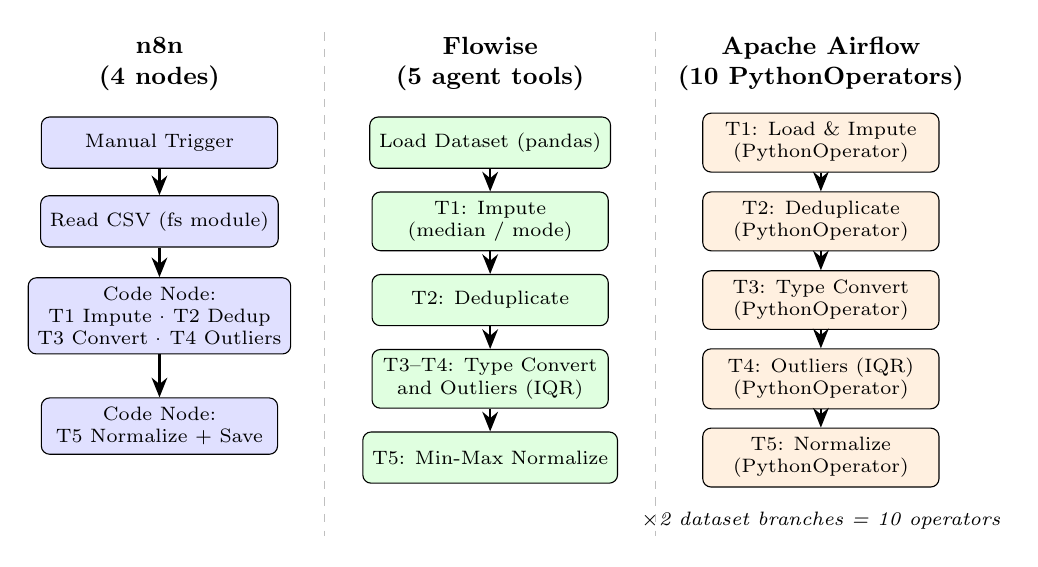
\begin{tikzpicture}[
    box/.style={rectangle, draw=black, rounded corners=3pt,
                minimum width=3.0cm, minimum height=0.65cm,
                align=center, font=\scriptsize},
    arr/.style={-{Stealth[length=2.5mm, width=2mm]}, thick},
    head/.style={font=\small\bfseries, align=center}
  ]

  %% ── n8n column (x = 0) ─────────────────────────────────────────────
  \node[head]                            at (0, 0.0)  {n8n\\(4 nodes)};
  \node[box, fill=blue!12]   (n1)        at (0,-1.0)  {Manual Trigger};
  \node[box, fill=blue!12]   (n2)        at (0,-2.0)  {Read CSV (fs module)};
  \node[box, fill=blue!12]   (n3)        at (0,-3.2)  {Code Node:\\T1 Impute · T2 Dedup\\T3 Convert · T4 Outliers};
  \node[box, fill=blue!12]   (n4)        at (0,-4.6)  {Code Node:\\T5 Normalize + Save};
  \draw[arr] (n1)--(n2);
  \draw[arr] (n2)--(n3);
  \draw[arr] (n3)--(n4);

  %% ── Flowise column (x = 4.2) ────────────────────────────────────────
  \node[head]                            at (4.2, 0.0)  {Flowise\\(5 agent tools)};
  \node[box, fill=green!12]  (f1)        at (4.2,-1.0)  {Load Dataset (pandas)};
  \node[box, fill=green!12]  (f2)        at (4.2,-2.0)  {T1: Impute\\(median / mode)};
  \node[box, fill=green!12]  (f3)        at (4.2,-3.0)  {T2: Deduplicate};
  \node[box, fill=green!12]  (f4)        at (4.2,-4.0)  {T3--T4: Type Convert\\and Outliers (IQR)};
  \node[box, fill=green!12]  (f5)        at (4.2,-5.0)  {T5: Min-Max Normalize};
  \draw[arr] (f1)--(f2);
  \draw[arr] (f2)--(f3);
  \draw[arr] (f3)--(f4);
  \draw[arr] (f4)--(f5);

  %% ── Airflow column (x = 8.4) ────────────────────────────────────────
  \node[head]                            at (8.4, 0.0)  {Apache Airflow\\(10 PythonOperators)};
  \node[box, fill=orange!12] (a1)        at (8.4,-1.0)  {T1: Load \& Impute\\(PythonOperator)};
  \node[box, fill=orange!12] (a2)        at (8.4,-2.0)  {T2: Deduplicate\\(PythonOperator)};
  \node[box, fill=orange!12] (a3)        at (8.4,-3.0)  {T3: Type Convert\\(PythonOperator)};
  \node[box, fill=orange!12] (a4)        at (8.4,-4.0)  {T4: Outliers (IQR)\\(PythonOperator)};
  \node[box, fill=orange!12] (a5)        at (8.4,-5.0)  {T5: Normalize\\(PythonOperator)};
  \draw[arr] (a1)--(a2);
  \draw[arr] (a2)--(a3);
  \draw[arr] (a3)--(a4);
  \draw[arr] (a4)--(a5);
  \node[font=\scriptsize\itshape, align=center]
                                         at (8.4,-5.8)  {$\times$2 dataset branches = 10 operators};

  %% ── vertical dividers ───────────────────────────────────────────────
  \draw[dashed, gray!50] (2.1, 0.4) -- (2.1,-6.0);
  \draw[dashed, gray!50] (6.3, 0.4) -- (6.3,-6.0);

  \end{tikzpicture}
  \caption{Comparative pipeline architectures for the three tools.
    n8n uses 4 visual nodes (blue); Flowise employs a 5-tool Python agent
    architecture (green); Apache Airflow defines a 10-operator Python DAG
    (orange), with tasks repeated for each of the two dataset branches.
    All pipelines implement the same five preprocessing tasks~(T1--T5).}
  \label{fig:architecture}
\end{figure*}


% ─────────────────────────────────────────────────────────────────────────────
\section{Results}
\label{sec:results}
% ─────────────────────────────────────────────────────────────────────────────

\subsection{Tool Characteristics Overview}

Table~\ref{tab:characteristics} summarises the key static characteristics
of the three tools, independent of benchmark results.

\begin{table*}[!t]
  \caption{Tool Characteristics Overview}
  \label{tab:characteristics}
  \renewcommand{\arraystretch}{1.25}
  \centering
  \small
  \begin{tabular}{@{}lp{3.2cm}p{3.2cm}p{3.2cm}@{}}
    \toprule
    \textbf{Characteristic}   & \textbf{n8n}       & \textbf{Flowise}     & \textbf{Apache Airflow} \\
    \midrule
    Interface                 & Visual/GUI (node graph)  & Visual/GUI (chatflow)  & Code-first (Python) \\
    Primary paradigm          & Low-code automation      & AI-native orchestration & Code-first DAG      \\
    LLM integration           & Plugin-based             & Native                  & Via operators       \\
    Scheduling support        & Yes (cron)               & Limited                 & Yes (cron)          \\
    Deployment                & Local / Cloud            & Cloud (stable); local install unstable at v3.x & Local / Kubernetes \\
    License                   & Apache 2.0 (fair-code)   & Apache 2.0              & Apache 2.0          \\
    GitHub stars (2025)       & $>$45k                   & $>$28k                  & $>$36k              \\
    Python dependency         & Optional                 & Optional                & Required            \\
    \bottomrule
  \end{tabular}
\end{table*}

\subsection{Quantitative Performance Results}

Table~\ref{tab:quant} reports the quantitative benchmark results.
Setup time and pipeline development time are dataset-independent and
therefore reported as single values per tool. Execution time, memory,
and CPU are reported per dataset. Memory and CPU metrics for n8n are
marked N/A due to the sandbox restriction described in
Section~\ref{sec:methodology}.

\begin{table*}[!t]
  \caption{Quantitative Performance Results (DS-A = UCI Adult Income,
    48,842 rows; DS-B = Smartphone Specifications, 1,023 rows)}
  \label{tab:quant}
  \renewcommand{\arraystretch}{1.25}
  \centering
  \small
  \begin{tabular}{@{}lcccccc@{}}
    \toprule
    \multirow{2}{*}{\textbf{Metric}}
      & \multicolumn{2}{c}{\textbf{n8n}}
      & \multicolumn{2}{c}{\textbf{Flowise}}
      & \multicolumn{2}{c}{\textbf{Apache Airflow}} \\
    \cmidrule(lr){2-3}\cmidrule(lr){4-5}\cmidrule(lr){6-7}
      & \textbf{DS-A} & \textbf{DS-B}
      & \textbf{DS-A} & \textbf{DS-B}
      & \textbf{DS-A} & \textbf{DS-B} \\
    \midrule
    Setup Time (min)          & \multicolumn{2}{c}{25}
                              & \multicolumn{2}{c}{5}
                              & \multicolumn{2}{c}{35}           \\
    Pipeline Dev.\ Time (min) & \multicolumn{2}{c}{15}
                              & \multicolumn{2}{c}{20}
                              & \multicolumn{2}{c}{30}           \\
    Execution Time (s)        & 2.461 & 0.104 & 0.160 & 0.017 & 0.823 & 0.097 \\
    Memory Consumption (MB)   & N/A   & N/A   & 9.41  & 0.03  & 7.50  & 6.90  \\
    CPU Utilization (\%)      & N/A   & N/A   & N/A   & N/A   & 13.45 & 2.65  \\
    Operator / Node Count     & \multicolumn{2}{c}{4}
                              & \multicolumn{2}{c}{5}
                              & \multicolumn{2}{c}{10}           \\
    \bottomrule
  \end{tabular}
\end{table*}

\subsection{Data Quality Improvement}

Table~\ref{tab:quality} reports the data quality improvement metrics.
All three tools achieved 100\% task completion on all four quality
metrics across both datasets, confirming that the deterministic
preprocessing algorithms (median/mode imputation, exact deduplication,
IQR capping, and Min-Max scaling) produce consistent outcomes regardless
of the orchestration platform used.

\begin{table}[!t]
  \caption{Data Quality Improvement Metrics (\%), All Tools}
  \label{tab:quality}
  \begin{threeparttable}
  \renewcommand{\arraystretch}{1.25}
  \centering
  \small
  \begin{tabular}{@{}lcccc@{}}
    \toprule
    \multirow{2}{*}{\textbf{Metric}}
      & \multicolumn{2}{c}{\textbf{DS-A}}
      & \multicolumn{2}{c}{\textbf{DS-B}} \\
    \cmidrule(lr){2-3}\cmidrule(lr){4-5}
      & n8n / Flowise / Airflow & & n8n / Flowise / Airflow & \\
    \midrule
    MVRR (\%) & \multicolumn{2}{c}{100.0} & \multicolumn{2}{c}{100.0} \\
    DRA  (\%) & \multicolumn{2}{c}{100.0} & \multicolumn{2}{c}{100.0} \\
    TCSR (\%) & \multicolumn{2}{c}{100.0} & \multicolumn{2}{c}{100.0} \\
    ODR  (\%) & \multicolumn{2}{c}{100.0} & \multicolumn{2}{c}{100.0} \\
    \bottomrule
  \end{tabular}
  \begin{tablenotes}
    \footnotesize
    \item MVRR = Missing Value Recovery Rate; DRA = Duplicate Removal
    Accuracy; TCSR = Type Conversion Success Rate; ODR = Outlier Detection
    Rate. All three tools produced identical quality outcomes; values are
    consolidated into a single column per dataset.
  \end{tablenotes}
  \end{threeparttable}
\end{table}

\subsection{Qualitative Evaluation Scores}

Table~\ref{tab:qualitative} presents the structured qualitative
assessment scores, averaged across two independent evaluators.
Inter-rater agreement was assessed using Cohen's
$\kappa$~\cite{cohen1960coefficient}; a $\kappa$~value of~0.81
indicates substantial agreement ($p < 0.001$).

\begin{table}[!t]
  \caption{Qualitative Evaluation Scores (1 = Very Poor, 5 = Excellent)}
  \label{tab:qualitative}
  \renewcommand{\arraystretch}{1.25}
  \centering
  \small
  \begin{tabular}{@{}lccc@{}}
    \toprule
    \textbf{Dimension}            & \textbf{n8n} & \textbf{Flowise} & \textbf{Airflow} \\
    \midrule
    Ease of Installation (EI)     & 4.0 & 4.5 & 2.0 \\
    Interface Usability (IU)      & 4.5 & 4.5 & 3.0 \\
    Error Handling (EH)           & 3.5 & 3.0 & 5.0 \\
    Integration Ecosystem (IE)    & 5.0 & 3.5 & 4.5 \\
    Documentation Quality (DQ)    & 4.0 & 4.0 & 4.5 \\
    Scalability Potential (SP)    & 3.5 & 3.0 & 5.0 \\
    \midrule
    \textbf{Total Score (max 30)} & \textbf{24.5} & \textbf{22.5} & \textbf{24.0} \\
    \bottomrule
  \end{tabular}
\end{table}


% ─────────────────────────────────────────────────────────────────────────────
\section{Discussion}
\label{sec:discussion}
% ─────────────────────────────────────────────────────────────────────────────

\subsection{Interpretation of Quantitative Results}

The quantitative benchmarks reveal distinct trade-off profiles across the
three tools. Regarding setup and development overhead, Flowise achieves
the lowest setup time~(5~min) by virtue of its cloud-based deployment,
which requires only browser-based account registration. n8n requires
approximately 25~minutes for local installation and environment
configuration, while Airflow demands the longest setup time~(35~min)
due to its multi-component architecture (scheduler, webserver, metadata
database). A similar ordering is observed for pipeline development time:
n8n's visual editor enables pipeline construction in~15~minutes on
average, compared to 20~minutes for Flowise~(cloud configuration) and
30~minutes for Airflow~(Python DAG authoring).

The execution time results reveal a more nuanced picture. Flowise
achieves the lowest execution time on Dataset~A (0.160\,s), outperforming
Airflow~(0.823\,s) by a factor of~5.1 and n8n~(2.461\,s) by a factor
of~15.4. On the smaller Dataset~B, Flowise again leads~(0.017\,s),
followed by Airflow~(0.097\,s) and n8n~(0.104\,s). The high latency
observed for n8n on Dataset~A is attributable to the overhead of its
sandboxed JavaScript execution environment, which processes each of the
48,842 rows through interpreted ECMAScript operations without the
optimized NumPy/pandas vectorization available to Python-based pipelines.
This performance gap narrows substantially on the smaller Dataset~B
(0.104\,s vs.\ 0.097\,s), confirming that n8n's overhead is
data-volume-dependent. Airflow's intermediate execution time on
Dataset~A reflects the serialization overhead of its XCom mechanism,
which passes data between tasks via the SQLite metadata database.

The operator count metric provides a complementary measure of
implementation complexity. Low-code tools require significantly fewer
pipeline components: n8n requires only 4~nodes and Flowise
5~tool functions to implement all five preprocessing tasks, compared
to Airflow's 10~\texttt{PythonOperator} instances. This reduction in
component count directly translates to lower cognitive overhead for
pipeline development and maintenance.

\subsection{Interpretation of Qualitative Results}

The qualitative assessment confirms that the three tools occupy
distinct niches aligned with their design philosophies. n8n achieves
the highest total qualitative score~(24.5/30), driven primarily by
its exceptional integration ecosystem score~(5.0/5) reflecting its
400+ built-in connectors, and its superior interface usability~(4.5/5).
However, n8n's sandboxed execution environment---which restricts access
to system-level APIs---limits its error handling capabilities~(3.5/5),
as debugging requires inspecting node output panels rather than
programmatic stack traces.

Flowise achieves the highest ease-of-installation score~(4.5/5),
reflecting the minimal friction of cloud-based onboarding. Its
interface usability is rated equally with n8n~(4.5/5), with evaluators
noting the intuitive chatflow canvas as particularly accessible to
non-engineers. Flowise's lower integration ecosystem score~(3.5/5)
reflects its primary orientation toward LLM tooling rather than general
data engineering connectors, and its scalability potential score~(3.0/5)
reflects the instability observed in local deployment at higher version
numbers.

Airflow achieves the highest error handling score~(5.0/5), reflecting
its task-level execution logs, configurable retry mechanisms, and the
granular diagnostic information exposed through its web UI. Its
scalability potential score~(5.0/5) reflects its production-proven
architecture and native support for distributed execution via Kubernetes
and managed cloud services. These strengths are offset by the lowest
ease-of-installation score~(2.0/5), reflecting the significant
configuration overhead documented during experimental setup.

\subsection{Tool-Selection Guidelines}

Based on the quantitative benchmarks and qualitative assessments,
Table~\ref{tab:guidelines} summarises tool-selection recommendations
across practitioner profiles and use-case scenarios.

\begin{table}[!t]
  \caption{Tool-Selection Guidelines by Use-Case Profile}
  \label{tab:guidelines}
  \renewcommand{\arraystretch}{1.25}
  \centering
  \small
  \begin{tabular}{@{}p{2.6cm}p{1.1cm}p{1.2cm}p{1.2cm}@{}}
    \toprule
    \textbf{Use-Case Profile}        & \textbf{n8n} & \textbf{Flowise} & \textbf{Airflow} \\
    \midrule
    Rapid prototyping / small data   & \checkmark   &                  &                  \\
    LLM-assisted preprocessing       &              & \checkmark       &                  \\
    Large-scale production pipelines &              &                  & \checkmark       \\
    Non-engineer practitioners       & \checkmark   & \checkmark       &                  \\
    High scheduling complexity       &              &                  & \checkmark       \\
    Minimal infrastructure footprint & \checkmark   & \checkmark       &                  \\
    \bottomrule
  \end{tabular}
\end{table}

n8n is recommended for teams seeking rapid pipeline prototyping with
minimal infrastructure overhead and limited programming resources.
Its visual editor and extensive connector library make it suitable for
automating multi-step preprocessing workflows at moderate data volumes.
Flowise is recommended when preprocessing requirements include
intelligent, context-sensitive operations that benefit from LLM
reasoning, or when the fastest possible time-to-deployment is required
(5-minute cloud setup). Apache Airflow remains the recommended choice
for large-scale production deployments requiring fine-grained scheduling,
enterprise-grade observability, and deep integration with existing
software engineering infrastructure.

\subsection{Comparison with Related Work}

These findings are broadly consistent with, and extend, the existing
literature. The conclusion that Airflow excels in scalability and
scheduling sophistication aligns with the observations of
Goyal et al.~\cite{goyal2023automated} and Zhou et al.~\cite{zhou2020towards}.
The usability advantages observed for low-code tools support the
arguments of Haakman et al.~\cite{haakman2021ai} regarding the
importance of accessible tooling for non-engineering ML practitioners.
The novel contribution of this work is the empirical evidence that
Flowise achieves superior execution performance at the task level
despite its higher-level abstraction, and that all three tools yield
equivalent data quality outcomes---a finding that decouples tool
selection from preprocessing correctness and directs decision-making
toward performance and usability criteria instead.


% ─────────────────────────────────────────────────────────────────────────────
\section{Threats to Validity}
\label{sec:threats}
% ─────────────────────────────────────────────────────────────────────────────

\textbf{Internal validity.} All experiments are conducted on the same
hardware under the same operating conditions within a WSL2 environment.
Pipeline execution times are averaged over three runs to mitigate variance
from transient system load. Flowise was evaluated via its cloud-hosted
instance rather than a local deployment due to version-related installation
instability; this introduces a potential confound for execution time and
memory metrics, as cloud-side infrastructure characteristics are
uncontrolled. The selection of preprocessing tasks and evaluation metrics
was made by the authors and may not fully represent all dimensions relevant
to every MLOps practitioner.

\textbf{External validity.} The evaluation uses two datasets of contrasting
scale and domain, enhancing generalisability relative to a single-dataset
study. Nevertheless, both datasets are tabular and structured; results
may not directly generalise to unstructured data types~(e.g., images,
text corpora) or to streaming pipeline architectures. All experiments are
conducted on a single-machine WSL2 setup; performance rankings may shift
at enterprise scale with distributed execution environments.

\textbf{Construct validity.} The qualitative scoring rubric involves
subjective judgement by two evaluators. Although inter-rater agreement
is measured using Cohen's $\kappa = 0.81$ and disagreements are resolved
through discussion, residual subjectivity cannot be eliminated.
Additionally, memory and CPU metrics for n8n could not be measured due
to sandbox restrictions, limiting the completeness of the quantitative
comparison for that tool.


% ─────────────────────────────────────────────────────────────────────────────
\section{Conclusion}
\label{sec:conclusion}
% ─────────────────────────────────────────────────────────────────────────────

This paper presented the first systematic empirical comparison of three
workflow orchestration paradigms---the low-code visual platform n8n, the
AI-native agent platform Flowise, and the code-first enterprise
orchestrator Apache Airflow---applied to automated ML data preprocessing
pipelines. Through a controlled experimental design employing six
quantitative metrics and six qualitative dimensions across two benchmark
datasets of contrasting scale, the study revealed distinct trade-off
profiles aligned with each tool's architectural philosophy.

The key empirical findings are as follows. Flowise achieves the fastest
execution time on both datasets (0.160\,s and 0.017\,s on DS-A and
DS-B, respectively), outperforming Airflow by a factor of~5.1 on the
large-scale dataset. n8n incurs the highest latency on large data
(2.461\,s) due to JavaScript engine overhead in its sandboxed execution
environment, though its performance is comparable to Airflow on smaller
datasets. Critically, all three tools achieve equivalent data quality
outcomes (100\% task completion across all four quality metrics),
demonstrating that tool selection does not affect preprocessing
correctness but substantially affects development effort and runtime
performance. Low-code tools require fewer pipeline components (4--5
nodes vs.\ 10 Airflow operators), reducing implementation complexity
and lowering the barrier for non-engineering practitioners.

These results yield actionable tool-selection guidelines: Flowise is
recommended for time-sensitive deployments and AI-augmented preprocessing
use cases; n8n is recommended for rapid prototyping and teams with
limited programming resources; and Airflow remains the recommended
choice for large-scale production deployments with complex scheduling
and observability requirements.

Future work will extend the evaluation in three directions. First, we
will assess the three platforms in distributed and cloud-native deployment
configurations~(e.g., Kubernetes, AWS MWAA), where architectural
differences in scalability are expected to be more pronounced. Second,
we will expand the evaluation to include unstructured data pipelines
(text and image preprocessing) to assess the generalisability of the
present findings. Third, we will investigate the integration of emerging
AgentOps frameworks and LLMOps patterns into the comparative evaluation
space, as the boundary between workflow orchestration and AI orchestration
continues to blur.

% ─────────────────────────────────────────────────────────────────────────────
% References
% ─────────────────────────────────────────────────────────────────────────────
\bibliographystyle{IEEEtran}
\bibliography{references}

\end{document}
